\subsection{Transfer Function}
\centerline{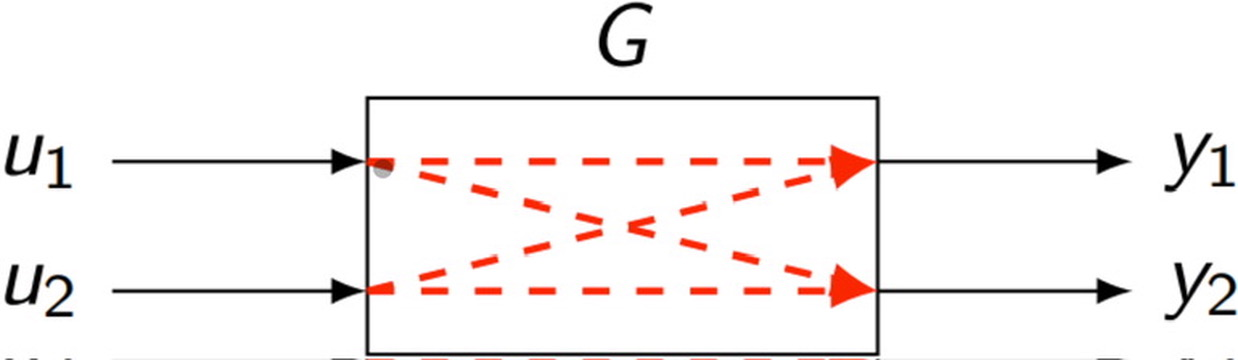
\includegraphics[width=0.5\linewidth]{src/6_mimo/images/transfer_function.jpeg}}

\begin{minipage}{0.55\linewidth}
    \vspace{1pt}
    \begin{equation*}
        \begin{pmatrix}
            y_1 \\
            y_2
        \end{pmatrix} =
        \begin{pmatrix}
            G_{11} & G_{12} \\
            G_{21} & G_{22}
        \end{pmatrix}
        \begin{pmatrix}
            u_1 \\
            u_2
        \end{pmatrix}
    \end{equation*} 
\end{minipage}
\begin{minipage}{0.44\linewidth}
    \begin{equation*}
        G(s) = \begin{pmatrix}
            G_{11} & G_{12} \\
            G_{21} & G_{22}
        \end{pmatrix}
    \end{equation*}
\end{minipage}
\vspace*{0.5em}

\textbf{Push through identity}
\vspace*{-0.5em}
$$
    G_1(I + G_2 G_1)^{-1} = (I + G_1 G_2)^{-1} G_1
$$

\textbf{MIMO state space to tf}
\vspace*{-0.5em}
$$
    G(s) = C(sI - A)^{-1}B + D
$$